%! Author = joels
%! Date = 27/01/2022

\section{Parser Einführung}
\textbf{$\rightarrow$ Kümmert sich um die syntaktische Analyse}\\
\textbf{Input:} Folge von Terminalsymbolen (Tokens)\\
\textbf{Output:} Syntaxbaum/Parse Tree\\
\textbf{Kontextfrei:} Parser beschränkt sich auf kontextfreie Sprachen (in EBNF beschreibbar). Kontextabhängige Aspekte wie Boolean lassen sich nicht addieren etc. übernimmt der Semantic Checker\\
\textbf{Aufgaben:}
\begin{itemize}[topsep=0pt]
    \itemsep -0.2em
    \item Finde eindeutige Ableitung der Syntaxregeln, um einen gegebenen Input herzuleiten
    \item Analysiert die gesamte Syntaxdefinition
    \item Erkennt, ob Eingabetext Syntax erfüllt oder nicht
    \item Eindeutige Ableitung erwünscht
    \item Erzeugt Syntaxbaum
\end{itemize}

\subsection{Concrete vs. Abstract Syntax Tree}
\textbf{Concrete:} Ableitung der Syntaxregeln als Baum widerspiegelt\\
\textbf{Abstract:} Unwichtige Details auslassen, Struktur vereinfachen und für Weiterverarbbeitung massschneidern\\
$\rightarrow$ Beides sind mögliche Intermediate Representations\\
$\rightarrow$ Generierter Parser kann Concrete Syntax Tree liefern\\
$\rightarrow$ Selbst implementierter Parser kann Abstract Syntax Tree liefern

\subsection{Parser Strategien}
\subsubsection{Top-Down}
\begin{itemize}[topsep=0pt]
    \itemsep -0.2em
    \item Beginne mit Start-Symbol
    \item Wende Produktionen an
    \item Expandiere Start-Symbol auf Eingabetext
    \SubItem{Expr -> Term + Term -> ... -> 1 + (2 - 3)}
\end{itemize}

\subsubsection{Buttom-Up}
\begin{itemize}[topsep=0pt]
    \itemsep -0.2em
    \item Beginne mit Eingabetext
    \item Wende Produktionen an
    \item reduziere Eingabetext auf Start-Symbol
    \SubItem{Expr <- Term + Term <- ... <- 1 + (2 - 3)}
\end{itemize}
\begin{minipage}{0,5\linewidth}
    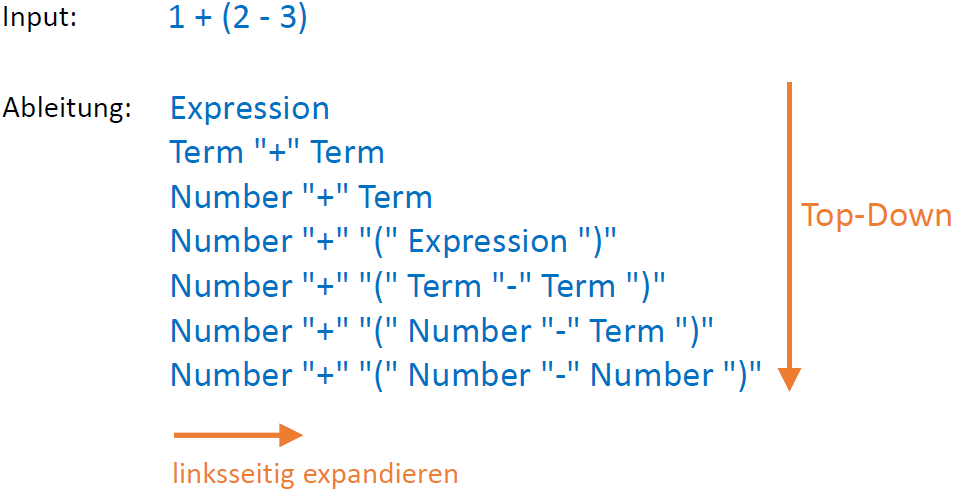
\includegraphics[width=\linewidth]{top_down_parser}
\end{minipage}
\begin{minipage}{0,5\linewidth}
    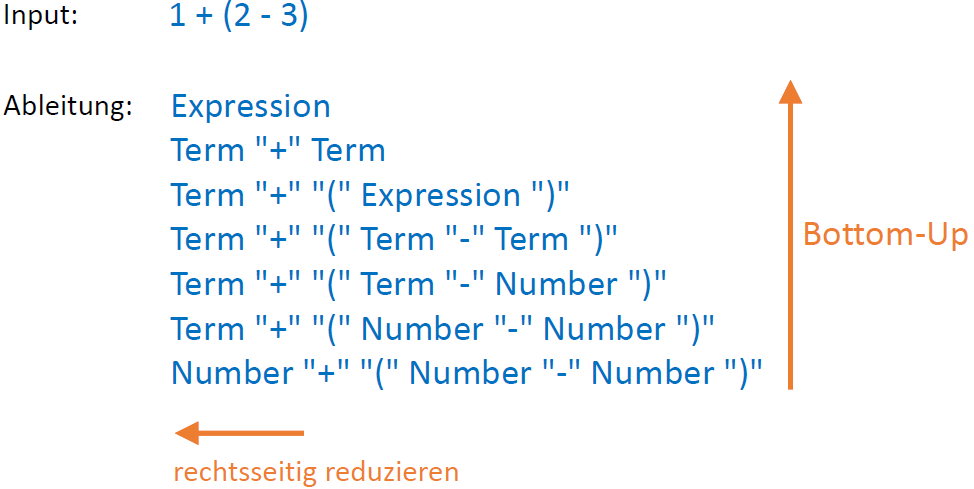
\includegraphics[width=\linewidth]{buttom_up_parser}
\end{minipage}

\subsubsection{Recoursive Descent}
\begin{itemize}[topsep=0pt]
    \itemsep -0.2em
    \item Pro Nicht-Terminalsymbol eine Methode
    \item Funktioniert bei rekursiven und nicht-rekursiven Produktionen
\end{itemize}
\textbf{Diskusion:}\\
\begin{itemize}[topsep=0pt]
    \itemsep -0.2em
    \item Recoursive Descent ist \textbf{Top-Down Parser}
    \SubItem{Implizierter Stack durch Methodenaufrufe}
    \SubItem{Entspricht Push-Down Automat}
    \item Zielorientierte Satzzerlegung (Predictive Direct)
    \SubItem{Immer klar, welche Produktion genommen wird, Bevorzugte Vorgehensweise}
    \item Anderer Ansatz: Backtracking
    \SubItem{Falls unklar welche Produktion zu nehmen ist: Wähle Produktion aus, bei Syntaxfehler Undo und nächste probieren}
\end{itemize}

\subsection{Implementation}
\subsubsection{Parser Gerüst}
\begin{lstlisting}
public class Parser {
    private final Iterator<Token> tokenStream;
    private Token current; // One Token lookahead

    private Parser(Iterable<Token> tokenStream) {
    this.tokenStream = tokenStream.iterator();
    }

    public static ProgramNode parse(Iterable<Token> stream) {
        return new Parser(stream).parseProgram();
    }
}
\end{lstlisting}

\subsubsection{Parser Einstieg}
\begin{lstlisting}
private ProgramNode parseProgram() {
    var classes = new ArrayList<ClassNode>();
    try {
        while (!isEnd()) {
            next();
            classes.add(parseClass());
        }
    } catch(IllegalArgumentException e) {
        error(e.getMessage());
    }
    return new ProgramNode(location, classes);
}
\end{lstlisting}

\subsection{Parsen mit längerem Lookahead}
\begin{lstlisting}
// Statement = Assignment | Invocation.
// Assignment = Identifier "=" Expression.
// Invocation = Identifier \dq(\dq \dq)\dq.

// Umwandeln zu:
// Statement = Identifier (AssignmentRest | InvocationRest).
// AssignmentRest = "=" Expression.
// Invocationrest = \dq(\dq \dq)\dq.

void parseStatement() {
    var identifier = readIdentifier();
    next();
    if (is(Tag.ASSIGN)) {
        parseAssignmentRest(identifier);
    } else if (is(Tag.OPEN_PARENTHESIS)) {
        parseInvocationRest(identifier);
    } else {
        error();
    }
}
\end{lstlisting}
